\documentclass[10pt]{beamer}

\usetheme{metropolis}
\usepackage{appendixnumberbeamer}
\usepackage[utf8]{inputenc}
\usepackage[spanish]{babel}
\usepackage{booktabs}
\usepackage[scale=2]{ccicons}
\usepackage{pgfplots}
\usepgfplotslibrary{dateplot}
\usepackage{xspace}
\usepackage{csquotes}
\usepackage{graphicx}
\usepackage{verbatim}
\usepackage{listings}

\newcommand{\themename}{\textbf{\textsc{metropolis}}\xspace}
\graphicspath{ {images/} }

\title{XVII Reunión de trabajo en Procesamiento de la Información y Control}
\subtitle{Modelando el patrón temporal del vector de dengue, Chikungunya y Zika
  a partir de información satelital con redes neuronales}

\date{Septiembre de 2017}

\begin{document}

\maketitle

\begin{frame}{Autores}
	\begin{alertblock}{UNC - FaMAF}
    Francisco C. Trucco, Juan M. Scavuzzo
	\end{alertblock}

	\begin{alertblock}{Instituto Gulich}
    Carolina B.Tauro
	\end{alertblock}

	\begin{alertblock}{Fundación Mundo Sano}
    Alba German, Manuel Espinosa, Marcelo Abril
	\end{alertblock}
\end{frame}

\setbeamercolor{background canvas}{bg=white}

\begin{frame}{Contenidos}
  \setbeamertemplate{section in toc}[sections numbered]
  \tableofcontents[hideallsubsections]
\end{frame}

\section{Introducción}

\begin{frame}{Epidemiología panorámica}

  \begin{itemize}[<+->]
  \item Factores ambientales de riesgo para la salud
  %% En la epidemiología panorámica se intenta comprender cuáles son los factores
  %% del medio ambiente que significan un riesgo para la salud del ser humano.
  \item Hasta hace poco: Exclusivamente con datos de campo
  %% Hasta hace poco tiempo ese estudio ecológico se realizaba exclusivamente con
  %% información recogida en el campo, tales como temperatura, precipitaciones,
  %% humedad relativa, salinidad, vegetación, fauna, entre otros.
  \item Hoy en día: Productos satelitales
  %% Pero hoy en día, se cuenta con una herramienta adicional de gran importancia y
  %% que define un nuevo concepto en la epidemiología, el uso de información e
  %% imágenes satelitales.
  \item[] \begin{center} \textbf{Epidemiología satelital} \end{center}

  \end{itemize}


\end{frame}

\begin{frame}{Epidemiología Satelital}
  \begin{center}
    \includegraphics[width=0.9\textwidth]{global.png}
  \end{center}
\end{frame}

\begin{frame}{Dengue, Zika y Chikungunya}

  \begin{itemize}[<+->]
  \item Enfermedades transmitidas por vectores
  %% Dengue, Zika y Chikungunya son enfermedades transmitidas por vectores.
  %% El dengue es una de estas enfermedades más importantes en el mundo.
  \item En América Latina el vector es el Aedes aegypti
  %% El vector de estas enfermedades en América Latina es el Aedes aegypti,
  %% mosquito peridoméstico que se cría preferentemente en contenedores
  %% artificiales.
  \item Aumento dramático de su incidencia
  %% La incidencia del dengue ha aumentado dramáticamente en las últimas décadas,
  %% con una tendencia creciente de brotes en Sudamérica en los últimos años. A
  %% esto se le suma la creciente incidencia del virus de chikungunya y zika.
  \end{itemize}

\end{frame}

\begin{frame}{Aprendizaje Automático (ML)}

    \begin{displayquote}[Tom Mitchell]
      A computer program is said to \textbf{learn} from experience $E$ with
      respect to some class of tasks $T$ and performance measure $P$, if its
      performance at tasks in $T$, as measured by $P$, improves with experience $E$
    \end{displayquote}


\end{frame}

\begin{frame}{Aprendizaje Automático (ML)}

  \begin{itemize}[<+->]
  \item Eficaz para clasificaciones y regresiones de sistemas \textbf{no
    lineales}
  %% El aprendizaje automático ha resultado ser un enfoque empírico eficaz para
  %% regresiones y clasificaciones de sistemas no lineales.
  \item Ideal para problemas con:
    \begin{itemize}
    \item Importante número de observaciones
    \item Conocimiento teórico incompleto
    \end{itemize}
  %% Por esto, el aprendizaje automático es ideal para abordar aquellos problemas
  %% donde se dispone de un número importante de observaciones, pero el conocimiento
  %% teórico es aún incompleto.
  \item Tiene gran número de aplicaciones en geociencias
    \begin{itemize}
    \item Océanos
    \item Atmósfera
    \item Algoritmos de extracción de información bio-geofisica
    \end{itemize}
  \end{itemize}

\end{frame}

\begin{frame}{Enfoques del Aprendizaje Automático}

  %% Los distintos enfoques del aprendizaje automático mayormente utilizados en
  %% geociencias y sensado remoto incluyen:

  \begin{itemize}[<+->]
  \item Linear Models
  \item Artificial Neural Networks
  \item Support vector machines
  \item K-Nearest Neighbour
  \item Decision trees
  \end{itemize}

\end{frame}

\begin{frame}{Las tres etapas de desarrollo de un modelo en ML}
  \begin{itemize}[<+->]
  \item Arquitectura y ajuste de parámetros
  \item Entrenamiento y validación 
  \item Utilización del modelo con datos nuevos
  \end{itemize}
\end{frame}

\defverbatim[colored]\lstI{
\begin{lstlisting}[language=Python]
  KNeighborsRegressor(n_neighbors, weights, algorithm,
                      leaf_size, p, metric,
                      metric_params, n_jobs, **kargs)
\end{lstlisting}
}

\begin{frame}{Ajuste de parámetros}
  \begin{itemize}[<+->]
  \item Algunos modelos dependen de parámetros.

  \item Ejemplo: \textbf{Ridge Regression}

  \item[] $$\hat{y}(w, x) = w_0 + w_1 x_1 + ... + w_p x_p$$

  \item[] $$\underset{w}{min\,}{{||X w - y||_2}}^2 + \alpha{||w||_2}^2$$

  \item Algunos modelos tienen aún más parámetros...

  \item[] \lstI

  \end{itemize}

\end{frame}

\begin{frame}{Entrenamiento y Validación}

  \begin{itemize}[<+->]
  \item Ejemplo: \textbf{Ridge Regression}

  \item[] $$\hat{y}(w, x) = w_0 + w_1 x_1 + ... + w_p x_p$$

  \item[] $$\underset{w}{min\,}{{||X w - y||_2}}^2 + \alpha{||w||_2}^2$$

  \item Se obtienen las variables del modelo

  \item Pero... ¿qué tan bueno es modelo según \textbf{cierta medida}?

  \item (Datos de entrenamiento, Datos de validación) 

  \item \textbf{Problema}: Los resultados pueden depender de una selección particular de
    este par

  \item \textbf{Solución}: Cross validation

  \end{itemize}
\end{frame}

\section{Herramientas}

\begin{frame}{Scikit Learn}

  Scikit Learn es una librería de Python para aprendizaje automático que
  implementa muchos algoritmos de clasificación y regresión.

  ¿Por qué Python? ¿Por qué esta librería?

  \stepcounter{beamerpauses}
  \begin{itemize}[<+->]
  \item Muy usado en el ámbito científico
  %% Python es uno de los lenguajes que han presenciado un crecimiento
  %% formidable en el ámbito académico en los últimos años además de ser uno de
  %% los más usados
  \item Tanto Python como Scikit Learn son software libre
  \item Hay una comunidad muy activa
  \item Fáciles de usar
  \end{itemize}

  %% Usamos el envi para obtener resultados de manera exploratoria
  %% Python es mucho más flexible para este tipo de problemas
  %% Uno de los objetivos de este trabajo fue usar algoritmos y herramientas
  %% \textbf{off-the-shelf}

\end{frame}

\begin{frame}{Iterated Racing for Automatic Algorithm Configuration (iRace)}
  \begin{itemize}[<+->]
  \item Ajusta los parámetros automáticamente
    %% Procedimiento iterativo capaz de encontrar automáticamente la
    %% configuración más adecuada de parámetros dado un conjunto de instancias
    %% del problema de optimización
  \item Realiza una búsqueda inteligente en el espacio de parámetros
  \item Muy útil para selección y comparación de modelos
  %% Dado que es crucial reducir el cesgo al comparar diferentes algoritmos, el
  %% ajuste de parámetros manual no es ideal.
  \item Implementada en R
  \item Software libre 
  \item Ha sido utilizada en trabajos similares
  \end{itemize}
\end{frame}

\section{Área de estudio}

\begin{frame}{Área de estudio: Tartagal}
  \begin{center}
  \includegraphics[width=0.9\textwidth]{tartagal.jpeg}
  \end{center}
  %% La Ciudad de Tartagal se encuentra en la base de las sierras subandinas
  %% argentinas en la provincia de Salta. La ciudad está rodeada de bosques nativos
  %% subtropicales y cultivos. El clima es subtropical.

\end{frame}

\section{Sistema Integral de Datos}
\begin{frame}{Sistema}
  \begin{center}
    \includegraphics[width=0.7\textwidth]{sistema.png}
  \end{center}

\end{frame}


\section{Modelos}

\begin{frame}{Variables}
  \includegraphics[width=1\textwidth]{all_variables.png}

  %% El uso de ovitrampas constituye un método efectivo para proporcionar datos
  %% útiles sobre la distribución espacial y temporal del Aedes aegypti.
  %% Se usaron productos satelitales que se analizaron influyentes para el
  %% medioambiente del mosquito según análisis de nuestro equipo de trabajo.

\end{frame}

\begin{frame}{Variables}

  %% De todas las variables ambientales recolectadas, solo algunas fueron
  %% seleccionadas como entradas del modelo.

  \includegraphics[width=1\textwidth]{selected_variables.png}

  %% Cabe aclarar que futuros trabajos pueden mejorar la selección de
  %% características para obtener mejores resultados.

\end{frame}

\begin{frame}{Modelos Lineales}
  \includegraphics[width=\textwidth]{lineal1.png}
\end{frame}

\begin{frame}{Modelos Lineales}
  \includegraphics[width=\textwidth]{lineal2.png}
\end{frame}

\begin{frame}{Modelos Lineales}
  \includegraphics[width=\textwidth]{lineal3.png}
\end{frame}

\begin{frame}{Modelos Lineales}
  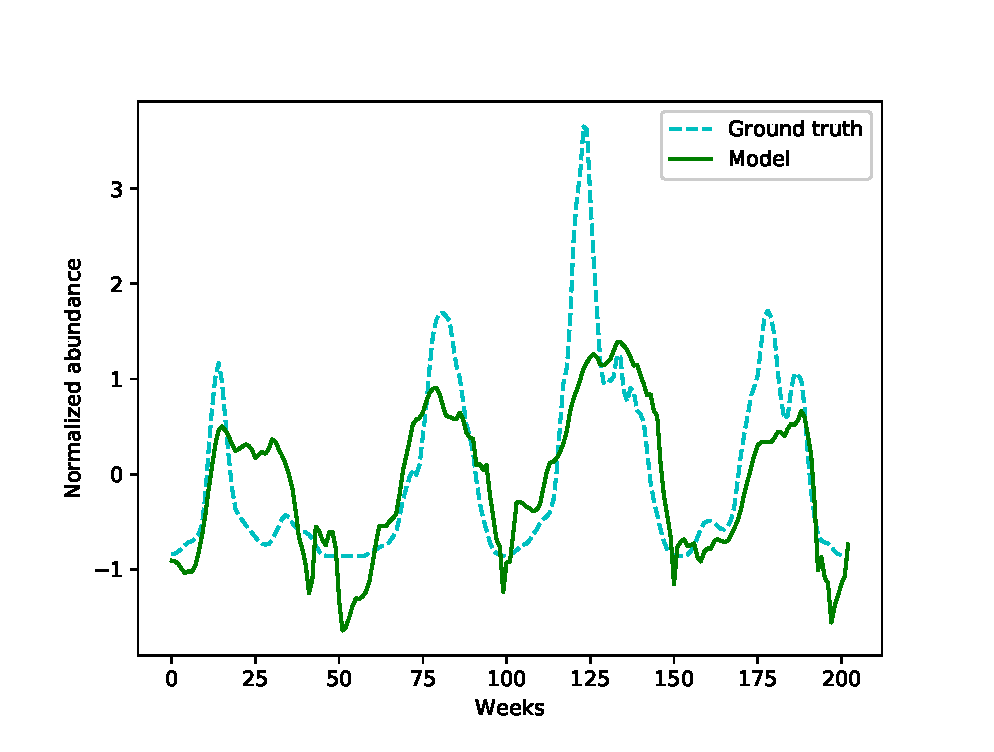
\includegraphics[width=\textwidth]{linear.eps}
\end{frame}

\begin{frame}{Modelos}
  \begin{center}
    \textbf{¿Son las regresiones lineales las más adecuadas para modelar este
      tipo de problemas?}
  \end{center}
\end{frame}

\section{Resultados}

\begin{frame}{Resultados: Support Vector Machine Regressor}
  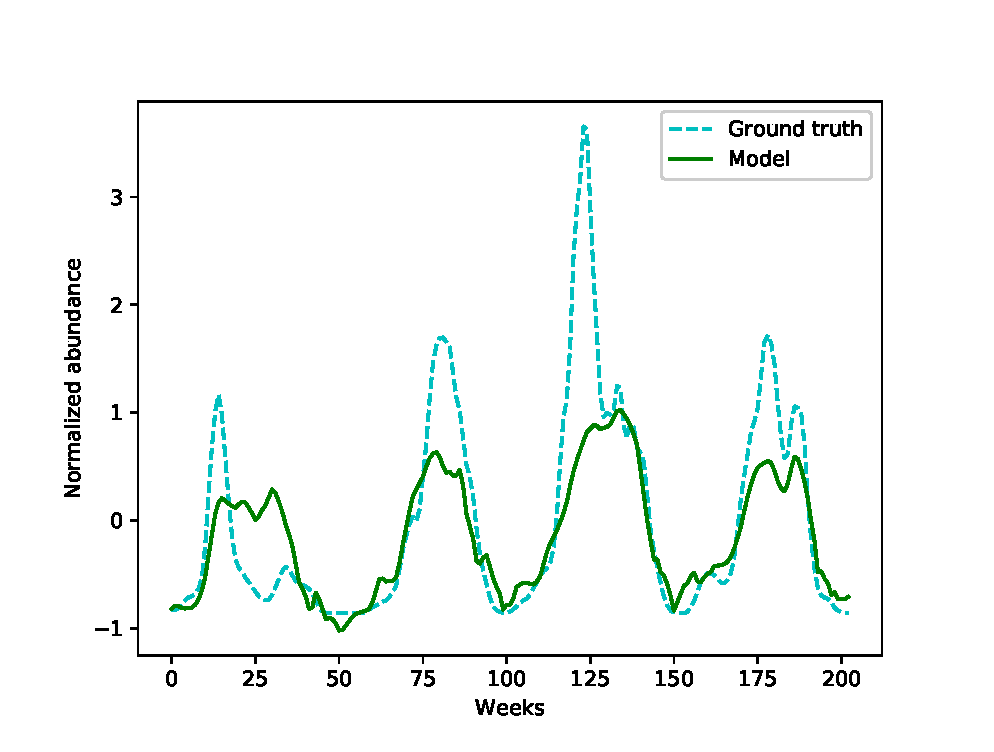
\includegraphics[width=\textwidth]{svr.eps}
\end{frame}

\begin{frame}{Resultados: Decision Tree}
  \includegraphics[width=\textwidth]{dtr.eps}
\end{frame}

\begin{frame}{Resultados: K-Nearest Neighbour}
  \includegraphics[width=\textwidth]{knnr1.eps}
\end{frame}

\begin{frame}{Resultados: Multi-layer Perceptron Regressor}
  \includegraphics[width=\textwidth]{mlpr.eps}
\end{frame}

\begin{frame}{Resultados: Comparación de modelos}
  \begin{center}
  \includegraphics[width=0.75\textwidth]{scatterplot.png}
  \end{center}
\end{frame}

\section{Conclusión}

\begin{frame}{Conclusión}
  \begin{itemize}[<+->]
    \item No Lineales vs Lineales

    \item Herramientas off-the-shelf
      %% Los modelos no lineales funcionan mejor que los modelos lineales.
      %% Aunque los modelos no lineales involucran una mayor complejidad a la
      %% hora de implementarlos, existen muchas herramientas off-the-shelf que
      %% facilitan esta tarea.

    \item Técnicas pocas veces utilizadas en problemáticas epidemiológicas
      %% La gran perspectiva en la utilización de este tipo de herramientas en
      %% este campo. Introducir técnicas sofisticadas como las de aprendizaje
      %% automático, pocas veces utilizadas en problemáticas epidemiológicas.

    \item Modelos operativos en el ámbito de la epidemiología
      %% La intención es que con estas herramientas se pueda desarrollar un
      %% sistema que pueda ser utilizado para llevar a cabo políticas de salud
      %% pública. El trabajo fue proyectado de manera que pudiera ser articulado
      %% con otros esfuerzos tendientes a avanzar en las direcciones
      %% establecidas por un proyecto institucional cuyo objetivo es abordar la
      %% problemática de la epidemiología.
  \end{itemize}
\end{frame}

\begin{frame}{Trabajos futuros: Cómo mejorar los resultados}
    \begin{itemize}[<+->]
    \item Aumentando la cantidad de datos
    \item Haciendo una mejor selección de características
    \item Entrenando sobre otras ciudades
    %% Los dos primeros mejoran la capacidad predictiva del modelo
    %% El último permite que los modelos puedan ser aplicados a otras
    %% regiones geográficas.
    \end{itemize}
\end{frame}

\begin{frame}[standout]
  ¿Preguntas?
\end{frame}

\appendix

\end{document}

%% \begin{frame}{Blocks}
%%   Three different block environments are pre-defined and may be styled with an
%%   optional background color.

%%   \begin{block}{Default}
%%     Block content.
%%   \end{block}

%%   \begin{alertblock}{Alert}
%%     Block content.
%%   \end{alertblock}

%%   \begin{exampleblock}{Example}
%%     Block content.
%%   \end{exampleblock}
%%   \stepcounter{beamerpauses}
%%   \begin{itemize}[<+->]
%%     \item Hola
%%     \item Chau
%%   \end{itemize}
%% \end{frame}
